\chapter{The W boson}
    \chapterprecishere{
        ``Potentielle citation sans aucun rapport avec le sujet"\par\raggedleft--- \textup{Personne inconnue}, contexte à déterminer
    }
    
   
        
    	\section{The motivation for the W mass measurement}    
        Being one of the cornerstones of the \gls{sm}, the W boson is tightly connected to the other parameters of the theory. In the leading order of the perturbation theory the W mass depends only on the electroweak parameters \cite{Awramik}:
        \begin{equation}
        M_W=\sqrt{\frac{\pi \alpha}{\sqrt{2}G_F}}\frac{1}{\sin{\theta_W}},
        \end{equation}
        where $G_F$ stands for the Fermi constant. The factor $\sqrt{\frac{\pi \alpha}{\sqrt{2}G_F}} \approx 40$ GeV sets the lower edge for the possible W mass. Higher order corrections enter the equation in a following way:
        \begin{equation}
        M_W=\sqrt{\frac{\pi \alpha}{\sqrt{2}G_F}}\frac{1}{\sin{\theta_W}}\frac{1}{1+\Delta r},
        \end{equation}
        where $\Delta r $ contains the sum of all possible radiative corrections and depends also on other parameters of the \gls{sm}, first of all on top quark and Higgs boson masses. The correction term is also sensitive to possible \gls{bsm} effects.
        \begin{figure}
        	\label{fig::mw_cor}
        	\centering
        	\feynmandiagram [horizontal=a to b, layered layout] {
        		i1 -- [boson, edge label = \( W \)] a,
        		a -- [scalar, half left, , edge label = \( H \)] b,
        		a -- [boson] b,
        		b -- [boson, edge label = \( W \)] f1,
        	};
        		\;  \; \; \; 
        	\feynmandiagram [horizontal=a to b,  layered layout, baseline=(b)] {
        		i1 -- [boson, edge label = \( W \)] a,
        		a -- [fermion, half left, , edge label = \( t \)] b,
        		b -- [fermion, half left, , edge label = \( \bar b \)] a,
        		b -- [boson, , edge label = \( W \)] f1,
        	};
        	\caption{ Next-to-leading order diagrams for W boson propagator containing contributions from heavy quarks and the Higgs boson.}
        \end{figure}
    As it was mentioned in Chapter 1 the mass of the W boson is one of the input parameters of the \gls{sm}, so the predictions of the theory directly depend on how precisely we know parameter value. On the other hand, we can theoretically constrain the value of the W boson mass assuming the measured values of the other parameters. Fig. \ref{w_values} demonstrates that the uncertainty of the theoretical estimate for the W boson mass is about two times lower than that of the best available experimental measurement. This motivates the effort for a more precise experimental measurement in order to test the consistency of the \gls{sm}. Should the improved measurement reveal the inconsistency of the Standard Model - it would also allow to determine viable \gls{bsm} theories. 
    	\begin{figure}[htbp]
    	\begin{subfigure}[t]{0.48\textwidth}
    		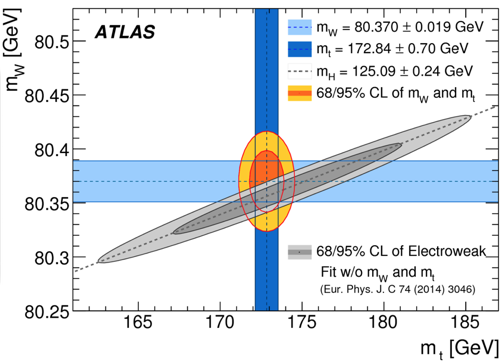
\includegraphics[width=\textwidth,keepaspectratio]{mw2.png}
    		\caption[Side view]{W mass constraint}
    		\label{fig::w_constraint}
    	\end{subfigure}
    	\hfill
    	\begin{subfigure}[t]{0.48\textwidth} 
    		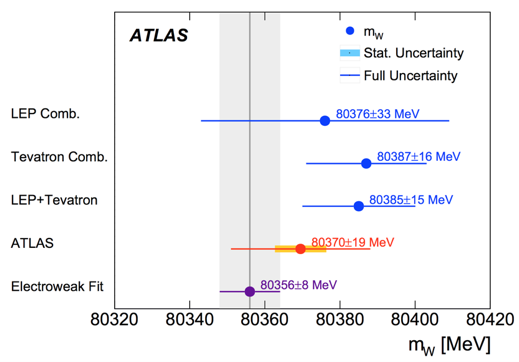
\includegraphics[width=\textwidth,keepaspectratio]{mw1.png}
    		\caption[Transverse view]{W mass measurements}
    		\label{fig::w_measurement}
    	\end{subfigure}
    	\caption{W mass measurements and predictions}
    	\label{fig::w_values}
    \end{figure}
        \section{Massive boson production at hadron colliders}
		Hadron colliders provide a fruitful environment for the production and study of massive electroweak bosons - all of them were discovered at hadron colliders. Hadron colliders allow to achieve much higher center-of-mass collision energy and luminosity comparing to their lepton counterparts. At the same time precision measurements at hadron colliers demand much deeper theoretical understanding of different aspects of the \gls{sm}. \\
		The main theoretical complication of the proton-proton colliders lies in the fact that in contrary to leptons, protons are complex objects. This raises the following new problems:
		\begin{itemize}
		\item It is not possible to take into account simultaneous interaction of many particles and find a solution for a many-body problem like a proton-proton collision.
		\item The initial energy of the whole proton is well known, but we don't know how this energy is distributed between the proton constituents.
		\end{itemize}
		In order to attack these problems and get accurate predictions for the proton-proton collisions it is necessary to take into account the asymptotic freedom that QCD demonstrates at short distances/high energies. At a certain energy scale of the momentum transferred during the collision $Q$ we can assume that the interacting parts of the proton are asymptotically free and neglect their interaction with the rest of the proton. This is called \textit{the factorization theorem} and only makes sense if the transferred momentum $Q\gg \Lambda_{QCD}$ is large enough, and that is why these processes are called "hard". The physical conditions of the hard processes allow to use the perturbative QCD formalism, since at large energy scale the strong coupling constant $\alpha_s$ becomes small. Processes with lower energy scale of the transferred momentum are called "soft" and do not allow to use the perturbative QCD formalism. As it was mentioned in Section 1, a lot of things in the low-energy non-perturbative sector of the QCD are still unclear. Nevertheless precise measurements at hadron colliders require certain understanding of both hard and soft QCD regimes.
		\subsection{Deep Inelastic scattering}
		In order to better understand the factorization approach let us first consider the lepton-hadron process called the \gls{dis}. Historically it was the first experimental evidence for the complex structure of the proton and still serves an indispensable tool for the proton structure study.
		\subsection{The Drell-Yan process}
		We can think of a proton (or any other hadron) as of a sum of 
		The bosons are produced via the \gls{dy} process. 
		\subsection{Soft QCD}
		
        \section{W boson detection}
        
		\section{W boson decay }

        \section{Precision measurements of WpT }

		\section{Precision measurements of W mass }

